\chapter{Future Work\authorB{}}

\textbf{Optimization and Industrialization:}
To enhance the industrial viability of this initiative, several essential measures must be implemented.
Foremost, there is a critical imperative to optimize bacterial proliferation efficiency and subsequent
Rare Earth Element (REE) yield. This necessitates the exploration of innovative methodologies aimed
at reducing growth duration and optimizing nutrient utilization by \emph{M. extorquens}.
Additionally, the substitution of methanol, the primary substrate for bacterial metabolism, with
methane, a more rudimentary and economically advantageous precursor, presents a promising
avenue, considering its compatibility with \emph{M. extorquens} metabolism.

For the full-scale industrialization of this project, comprehensive testing within large-scale bioreactor
systems is paramount. Concurrently, integration of diverse forms of electronic waste (e-waste) is
essential. Identifying the most economically viable categories of e-waste requires extensive
experimental evaluation. In parallel with these assessments, there is a pressing need for the
development of a high-capacity, efficient, and durable shredding apparatus specifically designed to
handle various types of E-Waste.

This endeavor poses multifaceted challenges, particularly regarding safety and cost considerations.
An industrial-grade E-Waste shredder must be inherently non-combustible and adept at processing
metal, plastic, fiberglass, and adhesive materials. Moreover, it must maintain optimal power
consumption levels and facilitate straightforward maintenance protocols. Such considerations are
integral to the successful implementation of sustainable and efficient recycling practices within
industrial contexts.

\textbf{Rare Earth Element Mining:}
\emph{Methylorubrum extorquens} (\emph{M. extorquens}) showcases remarkable Rare Earth Element (REE)
binding capabilities, presenting not only an avenue for e-waste recycling but also a potential
revolution in the mining of new REEs. Presently, traditional REE mining processes are notorious for
their heavy environmental footprint, characterized by significant pollution emissions.

\begin{figure}[H]
    \centering
    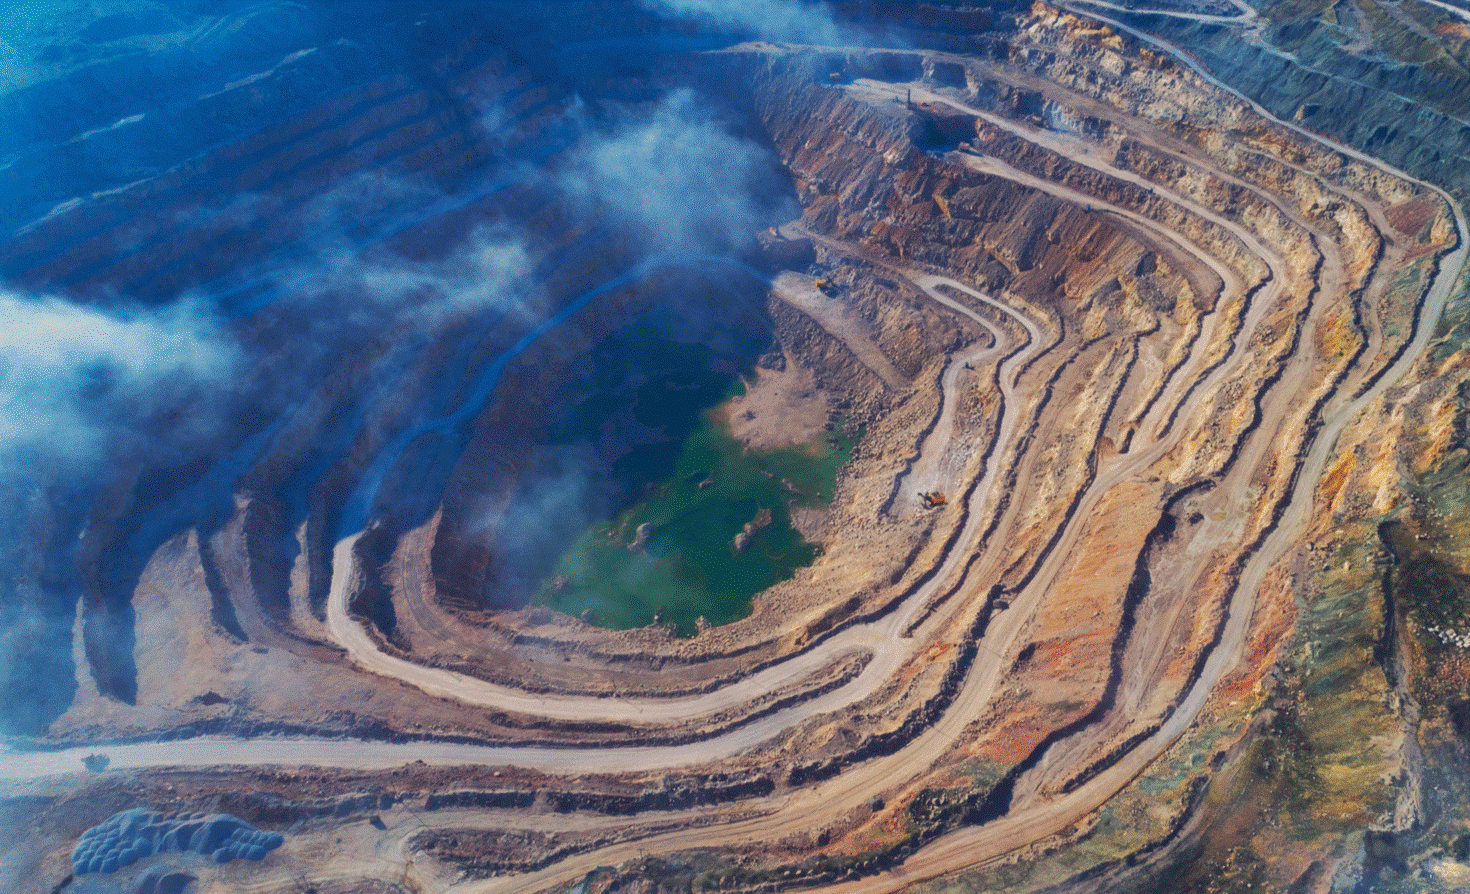
\includegraphics[width=0.8\textwidth]{./media/images/ree_mining_china}
    \caption{Rare earth element mining in China.}
    \label{fig:ree_mining_china}
\end{figure}

Unlike gold or iron, REEs are not typically found in large, concentrated deposits, necessitating
extensive excavation of ore-rich regions. Often, these sites contain ores with radioactive components
like uranium, adding another layer of environmental concern.

Following excavation, REEs are further concentrated through processes involving sulfuric acid.
Unfortunately, the liberation of REEs from minerals during this stage results in the release of sulfur
oxides, contributing significantly to acid rain formation. Moreover, the utilization of sulfuric acid,
along with hydrochloric and nitric acids for leaching REEs, poses substantial risks to both workers and
the environment.

The final critical step involves the separation of REEs from the acidic solution. Organophosphate
solvents such as tributyl phosphate (TBP) serve as selective host molecules, facilitating the dissolution
of REEs and their separation from aqueous solutions laden with impurities. However, TBP is known to
be toxic and persistent in the environment, posing significant safety concerns throughout its lifecycle.

In summary, the conventional REE extraction and refining processes are marred by severe pollution of
water and air. Ecosystems suffer disruption, aquatic life is adversely impacted, and human health is
jeopardized, underscoring the urgent need for alternative, more environmentally sustainable
approaches.

\textbf{Bioleaching:}
Utilizing lanmodulin's distinct properties, integral to our planned recycling initiative, we aim to
directly extract Rare Earth Elements (REEs) from ores. This methodology holds significant promise in
terms of cost reduction and environmental preservation by mitigating pollution. However, before
implementation, rigorous experimentation and validation are imperative. Factors such as efficiency,
bacterial survival within bioreactors in mining environments, and operational feasibility necessitate
thorough research and optimization. This can be achieved through localized trial runs in mines,
gradually integrating and refining our methods on a broader scale.